\documentclass[aspectratio=169,xcolor={dvipsnames,table}]{beamer}
\usepackage[no-math,deluxe,haranoaji]{luatexja-preset}
\renewcommand{\kanjifamilydefault}{\gtdefault}
\renewcommand{\emph}[1]{{\upshape\bfseries #1}}
\usetheme{metropolis}
\metroset{block=fill}
\setbeamertemplate{navigation symbols}{}
\usecolortheme[rgb={0.7,0.2,0.2}]{structure}
%%%%%%%%%%%%%%%%%%%%%%%%%%
%% Change alert block colors
%%% 1- Block title (background and text)
\setbeamercolor{block title alerted}{fg=mDarkTeal, bg=mLightBrown!45!yellow!45}
\setbeamercolor{block title example}{fg=magenta!10!black, bg=mLightGreen!70}
%%% 2- Block body (background)
\setbeamercolor{block body alerted}{bg=mLightBrown!25}
\setbeamercolor{block body example}{bg=mLightGreen!15}
%%%%%%%%%%%%%%%%%%%%%%%%%%%
%%%%%%%%%%%%%%%%%%%%%%%%%%%
\usepackage{media9}
%%%%%%%%%%%%%%%%%%%%%%%%%%%
%% さまざまなアイコン
%%%%%%%%%%%%%%%%%%%%%%%%%%%
\usepackage{fontawesome}
\usepackage{figchild}
\usepackage{twemojis}
\usepackage{utfsym}
\usepackage{bclogo}
\usepackage{marvosym}
\usepackage{tipa}
%%%%%%%%%%%%%%%%%%%%%%%%%%%
\usepackage{tikz}
\usetikzlibrary{backgrounds}
\usepackage{tcolorbox}
\usepackage{tikzpeople}
\usepackage{xcolor}
\usepackage{amsmath}
%%%%%%%%%%%%%%%%%%%%%%%%%%%
%% 場合分け
\usepackage{cases}
%%%%%%%%%%%%%%%%%%%%%%%%%%%
% \myAnch{<名前>}{<色>}{<テキスト>}
% 指定のテキストを指定の色の四角枠で囲み, 指定の名前をもつTikZの
% ノードとして出力する. 図には remeber picture 属性を付けている
% ので外部から参照可能である.
\newcommand*{\myAnch}[3]{%
  \tikz[remember picture,baseline=(#1.base)]
    \node[draw,rectangle,#2] (#1) {\normalcolor #3};
}
%%%%%%%%%%%%%%%%%%%%%%%%%%%%
%% 音声リンク表示
\newcommand{\myaudio}[1]{\href{#1}{\faVolumeUp}}
%%%%%%%%%%%%%%%%%%%%%%%%%%%
% \myEmph コマンドの定義
%\newcommand{\myEmph}[3]{%
%    \textbf<#1>{\color<#1>{#2}{#3}}%
%}
\usepackage{xparse} % xparseパッケージの読み込み
\NewDocumentCommand{\myEmph}{O{} m m}{%
    \def\argOne{#1}%
    \ifx\argOne\empty
        \textbf{\color{#2}{#3}}% オプション引数が省略された場合
    \else
        \textbf<#1>{\color<#1>{#2}{#3}}% オプション引数が指定された場合
    \fi
}
%%%%%%%%%%%%%%%%%%%%%%%%%%%
\title{English is fun.}
\subtitle{The Cat and the Mice}
\author{}
\institute[]{}
\date[]

%%%%%%%%%%%%%%%%%%%%%%%%%%%%
%% TEXT
%%%%%%%%%%%%%%%%%%%%%%%%%%%%
\begin{document}
%%%%%%%%%%%%%%%%%%%%%%%%%%%%
%%%%%%%%%%%%%%%%%%%%%%%%%%%%
\begin{frame}[label=waiting]{}
%%%%%\phantomsection\label{section}
\thispagestyle{empty}
\Large
\raggedright

予定の時刻になったらはじまります

\vfill

\raggedleft

The lesson will begin at the scheduled time.
\end{frame}
%%%%%%%%%%%%%%%%%%%%%%%%%%%%%
\begin{frame}[plain]
  \titlepage
\end{frame}

\section*{授業の流れ}
\begin{frame}[plain]
  \frametitle{授業の流れ}
  \tableofcontents
\end{frame}
%%%%%%%%%%%%%%%%%%%%%%%%%%%%%%%%%%%%%%%%%%%
\section{単数と複数}
%%%%%%%%%%%%%%%%%%%%%%%%%%%%%%%%%%%%%%%%%%%
\begin{frame}[plain]\frametitle{ひとつとふたつ以上}
\begin{columns}
\begin{column}{.25\textwidth}
\IfFileExists{./images/one_book-crop.pdf}{%
\rotatebox{-90}{\includegraphics[width=1.1\textwidth]{./images/one_book-crop.pdf}
}}{naiyo}
\end{column}\pause
\begin{column}{.5\textwidth}\LARGE
a book
\end{column}
\end{columns}

\pause
\begin{columns}
\begin{column}{.25\textwidth}
\IfFileExists{./images/two_books-crop.pdf}{%
\rotatebox{-90}{\includegraphics[width=1.1\textwidth]{./images/two_books-crop.pdf}
}}{naiyo}
\end{column}\pause
\begin{column}{.5\textwidth}\LARGE
two book\myEmph[4]{Maroon}{s}
\end{column}

\end{columns}
\end{frame}
%%%%%%%%%%%%%%%%%%%%%%%%%%%%%%%%%%
\subsection{日本語とのちがい}
%%%%%%%%%%%%%%%%%%%%%%%%%%%%%%%%%
\begin{frame}<1-10>[plain]\frametitle{日本語とのちがい}
\begin{columns}
\begin{column}[t]{.45\textwidth}
\begin{alertblock}{日本語}
\onslide<2->{わたしは1冊の本を持っています。}

\onslide<3->{わたしは2冊の本を持っています。}

\onslide<4->{わたしは本を持っています。}
\end{alertblock}
\end{column}
\begin{column}[t]{.45\textwidth}
\begin{block}{英語}
\onslide<5->{I have \textcolor{NavyBlue}{\bfseries a book.}}

\onslide<6->{I have \textcolor{NavyBlue}{\bfseries two books.}}

\onslide<7->*{I have \textcolor{Maroon}{\bfseries book}.}\onslide<8>{\,\,{}$\longleftarrow$これは\textcolor{Maroon}{だめ}}
\end{block}
\end{column}
\end{columns}

\begin{exampleblock}<9->{Topics for Today}
\begin{itemize}
 \item<1->  \onslide<9,10>{\textcolor{black}{単数形と複数形があります}}
 \item<2->  \onslide<10>{\textcolor{black}{単数形を裸で使うことはできません}}
\end{itemize}
      \end{exampleblock}

\end{frame}

\section{複数形のつくり方}
\subsection{基本}
\begin{frame}[plain]\frametitle{複数形のつくり方}
 
\Large
おしりに---sをつけます。

a book $\longrightarrow$ book\textcolor{Maroon}{s}

\end{frame}
%%%%%%%%%%%%%%%%%%%%%%%%%%%%%%%%%%%%%%
\subsection{Exercises}
\begin{frame}[plain]\frametitle{Exercises}

\fcDog{0.4}{black}{1}\pause {\large a dog}\hspace{30pt}%
\pause
\fcDog{0.4}{black}{1}\fcDog{0.4}{black}{1}\pause {\large two dog\textcolor{Maroon}{\bfseries s}}
\pause

\bigskip

\fcCat{0.4}{black}{1}\pause {\large a cat}\hspace{50pt}%
\pause
\fcCat{0.4}{black}{1}\fcCat{0.4}{black}{1}\fcCat{0.4}{black}{1} \pause {\large three cat\textcolor{Maroon}{\bfseries s}}
\pause

\bigskip

\fcBirdB{0.4}{black}{1}\pause {\large a bird}\hspace{55pt}%
\pause
\fcBirdB{0.4}{black}{1}
\fcBirdB{0.4}{black}{1}
\fcBirdB{0.4}{black}{1}
\fcBirdB{0.4}{black}{1} \pause {\large four bird\textcolor{Maroon}{\bfseries s}}

\myaudio{./audio/005_singular_plural_01.mp3}
\end{frame}
%%%%%%%%%%%%%%%%%%%%%%%%%%%%%%%%%%%%%%%%%%%%%%%%%%
\begin{frame}[plain]\frametitle{Exercises(Continued)}

\fcBookB{0.4}{black}{1}\pause {\large a book}\hspace{20pt}%
\pause
\fcBookB{0.4}{black}{1}\fcBookB{0.4}{black}{1}%
\fcBookB{0.4}{black}{1}\fcBookB{0.4}{black}{1}%
\fcBookB{0.4}{black}{1} \pause {\large five book\textcolor{Maroon}{\bfseries s}}
\pause

\bigskip

\scalebox{.17}{\fcKey{0.4}{black}{2}}\,\,{}\pause {\large a key}\hspace{40pt}%
\pause
\scalebox{.17}{\fcKey{0.4}{black}{2}} \scalebox{.17}{\fcKey{0.4}{black}{2}} \scalebox{.17}{\fcKey{0.4}{black}{2}} \scalebox{.17}{\fcKey{0.4}{black}{2}} \scalebox{.17}{\fcKey{0.4}{black}{2}} \scalebox{.17}{\fcKey{0.4}{black}{2}}
\pause
 {\large six key\textcolor{Maroon}{\bfseries s}}
\pause

\scalebox{.25}{\fcChairA{0.4}{black}{2}}\pause {\large a chair}\hspace{40pt}%
\pause
\scalebox{.25}{\fcChairA{0.4}{black}{2} \fcChairA{0.4}{black}{2} \fcChairA{0.4}{black}{2} \fcChairA{0.4}{black}{2} \fcChairA{0.4}{black}{2} \fcChairA{0.4}{black}{2} \fcChairA{0.4}{black}{2}}
\pause
 {\large seven chair\textcolor{Maroon}{\bfseries s}}
\pause

\scalebox{1}{\fcBike{0.4}{black}{1}}\pause {\large a bike}\hspace{30pt}%
\pause
\scalebox{1}{\begin{tabular}{@{}lllll}
\fcBike{0.4}{black}{1}& \fcBike{0.4}{black}{1}& \fcBike{0.4}{black}{1}& \fcBike{0.4}{black}{1}& \fcBike{0.4}{black}{1}\\
 \fcBike{0.4}{black}{1}& \fcBike{0.4}{black}{1}& \fcBike{0.4}{black}{1}
	     \end{tabular}}
\pause

\vspace*{-25pt}
\mbox{}\hspace*{.6\textwidth} {\large eight bike\textcolor{Maroon}{\bfseries s}}

\myaudio{./audio/005_singular_plural_02.mp3}
\end{frame}
%%%%%%%%%%%%%%%%%%%%%%%%%%%%%%%%%%%%%%%%%%%%%
\begin{frame}[plain]\frametitle{Exercises(Continued)}

\usymW{2710}{1cm}\pause {\large a pencil}\hspace{20pt}%
\pause
\usymW{2710}{1cm}\usymW{2710}{1cm}\usymW{2710}{1cm}\usymW{2710}{1cm}\usymW{2710}{1cm}\hspace{15pt}
\usymW{2710}{1cm}\usymW{2710}{1cm}\usymW{2710}{1cm}\usymW{2710}{1cm}\pause

\mbox{}\hspace{.8\textwidth} {\large nine pencil\textcolor{Maroon}{\bfseries s}}
\pause

\bcfleur\,\,\,\,\pause {\large a flower}\hspace{45pt}%
\pause
\bcfleur\bcfleur\bcfleur\bcfleur\bcfleur\hspace{15pt}
\bcfleur\bcfleur\bcfleur\bcfleur\bcfleur\hspace{10pt}
\pause
{\large ten flower\textcolor{Maroon}{\bfseries s}}

\myaudio{./audio/005_singular_plural_03.mp3}
\end{frame}
%%%%%%%%%%%%%%%%%%%%%%%
\begin{frame}[plain]\frametitle{Pronunciation}

\begin{enumerate}
 \item a dog~~~/~~~two dogs%
\hfill\makebox[40pt][l]{\textipa{/z/}}\hspace{180pt}\mbox{}
 \item a cat~~~/~~~three cats%
\hfill\makebox[40pt][l]{\textipa{/s/}}\hspace{180pt}\mbox{}
 \item a bird~~~~/~~~four birds%
\hfill\makebox[40pt][l]{\textipa{/z/}}\hspace{180pt}\mbox{}
 \item a book~~~/~~~five books%
\hfill\makebox[40pt][l]{\textipa{/s/}}\hspace{180pt}\mbox{}
 \item a key~~~/~~~six keys%
\hfill\makebox[40pt][l]{\textipa{/z/}}\hspace{180pt}\mbox{}
 \item a chair~~~/~~~seven chairs%
\hfill\makebox[40pt][l]{\textipa{/z/}}\hspace{180pt}\mbox{}
 \item a bike~~~/~~~eight bikes%
\hfill\makebox[40pt][l]{\textipa{/s/}}\hspace{180pt}\mbox{}
 \item a pencil~~~~/~~~nine pencils%
\hfill\makebox[40pt][l]{\textipa{/z/}}\hspace{180pt}\mbox{}
 \item a flower~~~/~~~ten flowers%
\hfill\makebox[40pt][l]{\textipa{/z/}}\hspace{180pt}\mbox{}
\end{enumerate}

% Embed the sound file
\pause
\mbox{}\hfill\myaudio{./audio/005_singular_plural_04.mp3}
\end{frame}
%%%%%%%%%%%%%%%%%%%%%%%%%%%%%%%%%%%%%%%%%%%%%
\subsection{注意すべき複数形}
%%%%%%%%%%%%%%%%%%%%%%%%%%%%%%%%%%%%%%%%%%%%%%
\begin{frame}[plain]{注意すべき複数形}

\scalebox{.5}{\fcBus{0.4}{black}{2}}\hspace{15pt}\pause {\LARGE a bus}
\pause

\bigskip

\bigskip

\scalebox{.5}{\fcBus{0.4}{black}{2}\hspace{15pt}\fcBus{0.4}{black}{2}}\hspace{15pt}
\pause {\LARGE two  bus\textcolor{orange}{es}}

\myaudio{./audio/005_singular_plural_05.mp3}\,\,{}Listen carefully.(注意して聞いてください)
\end{frame}
%%%%%%%%%%%%%%%%%%%%%%%%%%%%%%%%%%%%%%%%%%%%%%%%%%%%%%
\begin{frame}[plain]{注意すべき複数形}
\scalebox{.4}{\fcPotato{0.4}{black}{2}}\hspace{15pt}
\pause
{\LARGE a potato}
\pause

\bigskip

\bigskip

\scalebox{.4}{\fcPotato{0.4}{black}{2}\fcPotato{0.4}{black}{2}\fcPotato{0.4}{black}{2}}\hspace{15pt}
\pause
{\LARGE three  potato\textcolor{orange}{es}}

\myaudio{./audio/005_singular_plural_06.mp3}
\end{frame}
%%%%%%%%%%%%%%%%%%%%%%%%%%%%%%%%%%%%%%%%
\begin{frame}[plain]\frametitle{注意すべき複数形}

{\Large `s'ではなく\textcolor{orange}{`es'}をつける複数形があります}
\pause

\bigskip

\begin{block}{--- $\rightarrow$ ---es}

a bus \pause$\longrightarrow$ bus\textcolor{orange}{es}\pause%
\hfill\makebox[20pt]{\textipa{/iz/}}\hspace*{250pt}\pause

a class \pause$\longrightarrow$ class\textcolor{orange}{es}\pause
\hfill\makebox[20pt]{\textipa{/iz/}}\hspace*{250pt}\pause

a box \pause $\longrightarrow$ box\textcolor{orange}{es}\pause
\hfill\makebox[20pt]{\textipa{/iz/}}\hspace*{250pt}\pause

a potato \pause$\longrightarrow$ potato\textcolor{orange}{es}\pause
\hfill\makebox[20pt]{\textipa{/z/}}\hspace*{250pt}\pause

a tomato \pause$\longrightarrow$ tomato\textcolor{orange}{es}\pause
\hfill\makebox[20pt]{\textipa{/z/}}\hspace*{250pt}


\end{block}
\end{frame}
%%%%%%%%%%%%%%%%%%%%%%%%%%%%%%%%%%%%%%%%%%%%%%%%%%
\begin{frame}[plain]\frametitle{Pronunciation}

\begin{enumerate}
 \item a bus~~~\pause{}/~~~buses\pause
 \item a class~~~~\pause{}/~~~classes\pause
 \item a box~~~\pause{}/~~~boxes\pause
 \item a potato~~~\pause{}/~~~potatoes\pause
 \item a tomato~~~\pause{}/~~~tomatoes

 \end{enumerate}


\bigskip

\bigskip

\mbox{}\hfill\myaudio{./audio/005_singular_plural_07.mp3}
\end{frame}
%%%%%%%%%%%%%%%%%%%%%%%%%%%%%%%%%%%%%%%%%%%%%%%%%%%
\begin{frame}[plain]{注意すべき複数形}
\scalebox{5}{\ManFace}\hspace{15pt}
\pause
{\LARGE a man}
\pause

\bigskip

\bigskip

\scalebox{5}{\ManFace\hspace{5pt}\ManFace\hspace{5pt}\ManFace}\hspace{15pt}
\pause
{\LARGE three  \textcolor{orange}{men}}

\bigskip

\bigskip

\mbox{}\hfill\myaudio{./audio/005_singular_plural_08.mp3}
\end{frame}
%%%%%%%%%%%%%%%%%%%%%%%%%%%%%%%%%%%%%%%%%%%%%%%%%%%%%%%
\begin{frame}[plain]{注意すべき複数形}
\scalebox{5}{\WomanFace}\pause\hspace{15pt} {\LARGE a woman}
\pause

\bigskip

\bigskip

\scalebox{5}{\WomanFace \WomanFace \WomanFace \WomanFace} \hspace{25pt}
\pause
{\LARGE four  \textcolor{orange}{women}}

\bigskip

\bigskip

\mbox{}\hfill\myaudio{./audio/005_singular_plural_09.mp3}
\end{frame}
%%%%%%%%%%%%%%%%%%%%%%%%%%%%%%%%%%
\begin{frame}[plain]{注意すべき複数形}
\scalebox{.7}{%
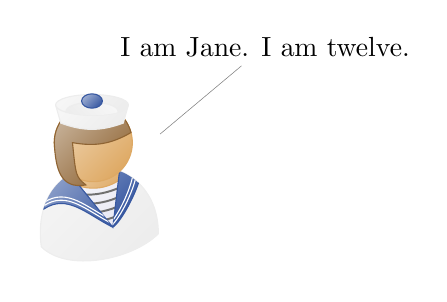
\begin{tikzpicture}
\node[sailor,female,minimum size=1.5cm,
anchor=south,pin={85:I am Jane. I am twelve.}] at (6.25cm,0) {};
%\node[charlie,minimum size=1.5cm,
%anchor=south,,pin={105:I am Bob.}] at (5cm,0) {};
\end{tikzpicture}
}\pause
\hspace{80pt}{\LARGE a child}
\pause

\bigskip

\scalebox{.7}{%
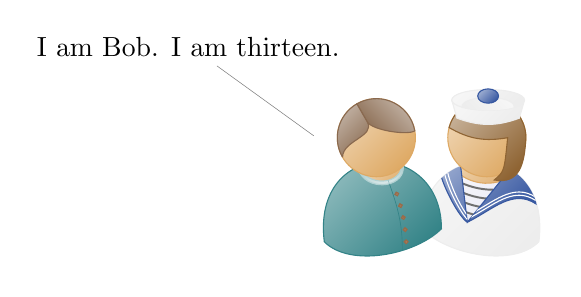
\begin{tikzpicture}
\node[sailor,female,mirrored,minimum size=1.5cm,
anchor=south] at (6.25cm,0) {};
\node[charlie,minimum size=1.5cm,
anchor=south,,pin={105:I am Bob. I am thirteen.}] at (5cm,0) {};
\end{tikzpicture}
}\pause
\hspace{45pt}{\LARGE two \textcolor{orange}{children}}

\bigskip

\bigskip

\mbox{}\hfill\myaudio{./audio/005_singular_plural_10.mp3}
\end{frame}
%%%%%%%%%%%%%%%%%%%%%%%%%%%%%%%%%%%%%%%%%%
\begin{frame}[plain]{注意すべき複数形}
 \fcMouse{.4}{gray}{.3}\pause\hspace{190pt}{\LARGE a mouse}

\bigskip

\bigskip

\fcMouse{.4}{gray}{.3}\fcMouse{.4}{gray}{.3}\fcMouse{.4}{gray}{.3}\fcMouse{.4}{gray}{.3}\pause\hspace{50pt}{\LARGE four \textcolor{Maroon}{\bfseries mice}}

\bigskip

\bigskip

\mbox{}\hfill\myaudio{./audio/005_singular_plural_11.mp3}
\end{frame}
%%%%%%%%%%%%%%%%%%%%%%%%%%%%%%%%%%%%%%%%%%
\begin{frame}[plain]\frametitle{Pronunciation}

\begin{enumerate}
 \item a man~~~\pause{}/~~~men\pause
 \item a woman~~~\pause{}/~~~women\pause
 \item a child~~~\pause{}/~~~children\pause
 \item a mouse~~~\pause{}/~~~mice
  \end{enumerate}
\pause

\bigskip

\bigskip

\mbox{}\hfill\myaudio{./audio/005_singular_plural_12.mp3}
\end{frame}
%%%%%%%%%%%%%%%%%%%
\end{document}
